% ============================================================
% Overcoming Vector Search Dilution in Scaled RAG Systems:
% A Multi-Agent Domain-Scoped Retrieval Architecture
% ============================================================
% Target: ACL / EMNLP / AAAI / SIGIR
% Format: ACL 2023+ compatible (also works with minor changes for AAAI, SIGIR)
% ============================================================

\documentclass[11pt,a4paper]{article}
\usepackage{acl}  % Official ACL style (acl.sty from acl-org/acl-style-files)
\usepackage{algorithm}
\usepackage{algorithmic}
\usepackage{tikz}
\usetikzlibrary{shapes,arrows,positioning,fit,calc}
\usepackage{pgfplots}
\pgfplotsset{compat=1.18}
\usepackage{listings}
\usepackage{booktabs}
\usepackage{multirow}
\usepackage{amsmath}
\usepackage{amssymb}
\usepackage{xcolor}
\usepackage{enumitem}
\usepackage{subcaption}
\usepackage{float}  % For [H] exact float placement

% Custom colors
\definecolor{agentblue}{RGB}{66,133,244}
\definecolor{routergreen}{RGB}{52,168,83}
\definecolor{dilutionred}{RGB}{234,67,53}
\definecolor{codebg}{RGB}{245,245,245}

% Custom commands
\newcommand{\systemname}{\textsc{MASDR-RAG}}
\newcommand{\todo}[1]{\textcolor{red}{\textbf{[TODO: #1]}}}
\newcommand{\fillme}[1]{\textcolor{blue}{\textbf{[FILL: #1]}}}
\newcommand{\numDocs}{1{,}128}
\newcommand{\numChunks}{88{,}907}

% Listings
\lstset{
  basicstyle=\ttfamily\small,
  backgroundcolor=\color{codebg},
  breaklines=true,
  frame=single,
  framerule=0.5pt,
  columns=fullflexible
}

% ============================================================
\title{Overcoming Vector Search Dilution in Scaled RAG Systems:\\
A Multi-Agent Domain-Scoped Retrieval Architecture\\for Government Document Collections}

\author{
  \textbf{Nabaraj Subedi}$^{1}$ \\
  $^{1}$Department of Computer Science, University of Wyoming \\
  \texttt{nsubedi1@uwyo.edu}
}

\date{}

\begin{document}
\maketitle

% ============================================================
% ABSTRACT
% ============================================================
\begin{abstract}
Retrieval-Augmented Generation (RAG) systems face a critical yet understudied failure mode when scaling document collections: \textit{vector search dilution}, where embedding similarity becomes progressively less discriminative as semantically adjacent but contextually irrelevant chunks proliferate across heterogeneous document categories. We present a systematic study of this phenomenon using a real-world deployment for the Wyoming Department of Transportation (WYDOT), where scaling from 54 to \numDocs{} documents (1,600 to \numChunks{} chunks) caused answer quality to degrade from 56\% to 58\% accuracy. We diagnose the root causes---vocabulary overlap across document categories and chunk distribution imbalance---and propose \systemname{} (\textbf{M}ulti-\textbf{A}gent \textbf{S}coped \textbf{D}omain \textbf{R}etrieval for \textbf{RAG}), an architecture combining LLM-based zero-shot query routing with domain-scoped retrieval over a Neo4j knowledge graph. Our approach reduces the effective search space by 85--95\% per query while achieving 100\% query coverage, compared to 37\% with rule-based routing. Experiments on 57 domain-expert-curated queries demonstrate that \systemname{} restores retrieval precision to pre-scaling levels while enabling new multi-hop capabilities not possible with monolithic retrieval. We release our architecture and evaluation framework to support future research on scaling RAG for large, heterogeneous document collections.\footnote{Code: \textit{Available upon publication}}
\end{abstract}

% ============================================================
% 1. INTRODUCTION
% ============================================================
\section{Introduction}
\label{sec:introduction}

Retrieval-Augmented Generation (RAG) has emerged as the dominant paradigm for grounding large language model (LLM) outputs in external knowledge \cite{lewis2020rag, guu2020realm}. By retrieving relevant passages from a document corpus before generation, RAG systems mitigate hallucination \cite{shuster2021retrieval, huang2023hallucination}, enable access to private or domain-specific data \cite{gao2024ragsurvey}, and avoid the prohibitive cost of fine-tuning \cite{izacard2023atlas}. The standard RAG pipeline---embed documents, build a vector index, retrieve top-$k$ similar chunks, feed to an LLM---works remarkably well for small, homogeneous corpora.

However, a critical gap exists between laboratory-scale RAG experiments, typically conducted on curated datasets of tens to hundreds of documents \cite{kwiatkowski2019naturalquestions, joshi2017triviaqa}, and production deployments that must serve thousands of heterogeneous documents. As organizations digitize their knowledge bases, RAG systems are increasingly tasked with handling diverse document collections spanning multiple domains, formats, and time periods \cite{barnett2024observations}. This scaling challenge is particularly acute in government and enterprise settings, where document collections grow by orders of magnitude during deployment \cite{rag4cm2025}.

In this paper, we identify and characterize \textit{vector search dilution}---a phenomenon where the discriminative power of embedding-based retrieval degrades as the document corpus scales across heterogeneous categories. Unlike the well-studied scalability challenges of approximate nearest neighbor (ANN) algorithms \cite{malkov2020hnsw, johnson2021faiss}, vector search dilution is a \textit{semantic} problem: as documents from different domains share overlapping vocabulary, embedding models produce similar vectors for semantically adjacent but contextually irrelevant chunks, causing top-$k$ retrieval to return cross-domain noise.

We ground our analysis in a real-world case study: a knowledge graph-powered RAG chatbot deployed for the Wyoming Department of Transportation (WYDOT). When the system scaled from 54 documents (1,600 chunks) to \numDocs{} documents (\numChunks{} chunks) across 9 document categories, answer quality degraded catastrophically---queries about construction specifications returned crash report statistics, and materials testing queries retrieved bridge design documents.

To address this, we propose \systemname{}, combining three innovations:

\begin{enumerate}[leftmargin=*,topsep=2pt,itemsep=1pt]
    \item \textbf{LLM-based zero-shot query routing}: A fast LLM call classifies each query into one of 10 document categories, achieving 100\% query coverage vs.\ 37\% with regex matching (\S\ref{sec:routing}).
    \item \textbf{Domain-scoped retrieval via knowledge graph metadata}: Each domain agent restricts search to document subsets defined by Neo4j graph metadata, reducing the effective search space by 85--95\% (\S\ref{sec:scoped_search}).
    \item \textbf{Multi-agent orchestration with tool calling}: A Gemini-based orchestrator uses function calling to dispatch queries to specialized agents, enabling multi-hop reasoning and cross-domain comparison (\S\ref{sec:orchestrator}).
\end{enumerate}

Our contributions are: (1) the first systematic diagnosis of vector search dilution in a production RAG system (\S\ref{sec:dilution}); (2) a complete architecture from diagnosis to solution combining LLM routing, graph-based scoping, and multi-agent orchestration (\S\ref{sec:architecture}); (3) evaluation on \numDocs{} real government documents across 9 categories (\S\ref{sec:evaluation}); and (4) practical guidelines for when dilution becomes critical and how to determine optimal agent granularity (\S\ref{sec:discussion}).


% ============================================================
% 2. RELATED WORK
% ============================================================
\section{Related Work}
\label{sec:related_work}

\subsection{Retrieval-Augmented Generation}

The RAG paradigm was formalized by \citet{lewis2020rag}, building on open-domain QA with retrieval \cite{chen2017drqa, karpukhin2020dpr}. REALM \cite{guu2020realm} introduced pre-training with retrieval, while Fusion-in-Decoder \cite{izacard2021fid} demonstrated effective multi-passage reasoning. Subsequent work explored atlas-scale pre-training \cite{izacard2023atlas}, retrieval-augmented language modeling \cite{borgeaud2022retro}, and RAG frameworks \cite{gao2024ragsurvey, zhao2024ragsurvey2}. The evolution from naive RAG to advanced RAG (with query transformation, re-ranking, and iterative retrieval) is well-documented \cite{gao2024ragsurvey}. Recently, the community has identified the transition toward \textit{agentic RAG} \cite{singh2025agenticrag}, where autonomous agents decide when, what, and how to retrieve. Our work falls in this agentic category but is motivated by a specific production failure mode.

\subsection{Dense Retrieval and Scaling}

Dense retrieval using learned embeddings \cite{karpukhin2020dpr, xiong2021ance} has largely supplanted sparse methods like BM25 \cite{robertson2009bm25} for semantic search, though hybrid approaches remain competitive \cite{chen2024blendedrag, ma2024hybridretrieval}. Embedding models evolved from Sentence-BERT \cite{reimers2019sentencebert} through instruction-tuned models \cite{su2023instructor} to large embedding models \cite{wang2024e5mistral, li2024bge}. Late interaction models like ColBERT \cite{khattab2020colbert} and ColBERTv2 \cite{santhanam2022colbertv2} offer finer-grained matching at higher cost. Learned sparse representations \cite{formal2021splade} bridge dense and sparse paradigms.

The scaling challenges of dense retrieval are typically framed in terms of ANN performance. HNSW \cite{malkov2020hnsw} trades recall for speed as index size grows. FAISS \cite{johnson2021faiss} and ScaNN \cite{guo2020scann} address computational efficiency. However, these focus on \textit{algorithmic} scalability. We identify a distinct \textit{semantic} scaling problem: even when ANN returns the true nearest neighbors, those neighbors may be irrelevant due to embedding space contamination by heterogeneous documents. This has received limited attention, with \citet{barnett2024observations} providing the most relevant production observations.

\subsection{Query Routing and Classification}

Adaptive-RAG \cite{jeong2024adaptiverag} routes queries by complexity. RAGRouter \cite{ragrouter2025} trains classifiers for strategy selection. Multi-Meta-RAG \cite{zohar2024multimetarag} uses metadata filtering for multi-hop queries. RouteRAG \cite{routerag2025} dynamically routes between strategies. Semantic routing \cite{aurelio2024semanticrouter} matches queries to route descriptions via embeddings. Query transformation methods complement routing: HyDE \cite{gao2023hyde} generates hypothetical documents, step-back prompting \cite{zheng2024stepback} abstracts queries, and decomposition \cite{press2023measuring, zhou2023leasttomost} breaks complex queries into sub-queries. Query2doc \cite{wang2023query2doc} uses LLMs to expand queries.

Our routing is distinct: (1) we route by \textit{document domain} rather than strategy or complexity, and (2) we use \textit{zero-shot LLM classification} rather than trained classifiers, eliminating the need for labeled training data.

\subsection{Multi-Agent LLM Systems}

ReAct \cite{yao2023react} interleaves reasoning and acting. Toolformer \cite{schick2023toolformer} teaches LLMs tool use. Function calling in commercial models enables practical architectures \cite{patil2023gorilla, qin2024toolllm}. Chain-of-thought \cite{wei2022chainofthought} and tree-of-thought \cite{yao2024treeofthoughts} provide structured reasoning. Planning with LLMs \cite{huang2022planning} enables complex task decomposition. AutoGen \cite{wu2023autogen} and CrewAI \cite{crewai2024} provide multi-agent frameworks.

In RAG, MA-RAG \cite{marag2025} uses multiple agents for retrieval/generation. \citet{multiagentrag2024} demonstrate collaborative agents for research tasks. The agentic RAG survey \cite{singh2025agenticrag} provides a taxonomy. A-RAG \cite{arag2026} explores autonomous retrieval agents. CRAG \cite{yan2024crag} implements corrective retrieval. Self-RAG \cite{asai2023selfrag} learns to critique its own retrieval.

Our agents serve as \textit{domain gatekeepers} rather than task specialists---each restricts search to a specific document subset, directly addressing dilution.

\subsection{Graph-Enhanced Retrieval}

Microsoft's GraphRAG \cite{edge2024graphrag} builds entity-relationship graphs and uses community detection for global queries. HybridRAG \cite{hybridrag2024} combines KG traversal with vector similarity. \citet{peng2024graphragsurvey} survey graph RAG approaches. KG-RAG \cite{soman2024kgrag} augments biomedical QA with knowledge graphs. GRAG \cite{grag2024} explores graph-structured retrieval. LightRAG \cite{guo2024lightrag} provides efficient graph-based retrieval. Knowledge graph construction using LLMs \cite{pan2024kgllm, trajanoska2023kgconstruction} has simplified entity extraction.

Our approach differs: we leverage the graph's \textit{organizational metadata} (document series, sections, supersession relationships) as agent boundaries, not entity relationships for retrieval.

\subsection{Domain-Specific RAG}

RAG has been applied to legal documents \cite{louis2024interpretable, pipitone2024legalrag}, medical QA \cite{xiong2024benchmarking, zakka2024almanac}, scientific literature \cite{press2023measuring}, financial analysis \cite{li2024finrag}, and construction management \cite{rag4cm2025}. \citet{graphragcompliance2024} apply graph-RAG to engineering compliance. Government documents present unique challenges: decades of versions, specialized overlapping terminology, and diverse user expertise levels.

\subsection{RAG Evaluation}

RAGAS \cite{es2024ragas} measures faithfulness, relevance, and context precision. ARES \cite{saadfalcon2024ares} provides automated evaluation. RGB \cite{chen2024rgb} benchmarks robustness. CRAG benchmark \cite{yang2024crag} tests comprehensive RAG capabilities. Standard benchmarks like Natural Questions \cite{kwiatkowski2019naturalquestions}, TriviaQA \cite{joshi2017triviaqa}, and MS MARCO \cite{nguyen2016msmarco} use homogeneous corpora and do not capture cross-domain dilution.

\subsection{Document Processing and Chunking}

Chunking strategies significantly impact retrieval \cite{langchain2024textsplitters}. Semantic chunking \cite{kamradt2024semantic} preserves coherence. Late chunking \cite{gunther2024latechunking} defers splitting. Parent document retrieval \cite{langchain2024parentdoc} retrieves larger contexts. RAPTOR \cite{sarthi2024raptor} builds hierarchical summaries for multi-resolution retrieval. Our analysis reveals that chunking interacts with dilution: statistical tables produce thousands of small chunks that flood the embedding space.


% ============================================================
% 3. VECTOR SEARCH DILUTION
% ============================================================
\section{Vector Search Dilution}
\label{sec:dilution}

\subsection{System Context}

WYDOT maintains \numDocs{} documents spanning construction specifications, design manuals, materials testing procedures, crash reports, transportation improvement programs, and administrative reports. These were ingested into a Neo4j knowledge graph:
\begin{equation}
\text{Document} \xrightarrow{\text{CONTAINS}} \text{Section} \xrightarrow{\text{CONTAINS}} \text{Chunk}
\end{equation}

Chunks were embedded using Google's Gemini Embedding model (\texttt{gemini-embedding-001}, 768 dimensions) and indexed via HNSW vector index plus BM25 fulltext index. The system uses hybrid search \cite{chen2024blendedrag} with Gemini 2.0 Flash for generation.

\begin{table}[H]
\centering
\resizebox{\columnwidth}{!}{%
\begin{tabular}{lrrrr}
\toprule
\textbf{Category} & \textbf{Docs} & \textbf{Chunks} & \textbf{\%} & \textbf{Chk/Doc} \\
\midrule
Standard Specs & 2 & 2,519 & 2.8 & 1260 \\
Construction Manual & 21 & 6,641 & 7.5 & 316 \\
Materials Testing & 6 & 2,180 & 2.5 & 363 \\
Design Manual & 23 & 1,405 & 1.6 & 61 \\
Traffic \& Crashes & 22 & 30,922 & 34.8 & 1406 \\
STIP & 59 & 13,634 & 15.3 & 231 \\
Annual Reports & 46 & 2,341 & 2.6 & 51 \\
Bridge Program & 28 & 5,399 & 6.1 & 193 \\
Highway Safety & 0 & 0 & 0.0 & 0 \\
Other & 921 & 23,866 & 26.8 & 26 \\
\midrule
\textbf{Total} & \numDocs & \numChunks & 100 & -- \\
\bottomrule
\end{tabular}%
}
\caption{Document and chunk distribution. Traffic \& Crash reports contribute 35.7\% of chunks despite being 2.0\% of documents. Chunk density (Chk/Doc) varies up to 54$\times$ across categories.}
\label{tab:distribution}
\end{table}

\subsection{Scaling and Degradation}

The system was deployed in two phases:
\begin{itemize}[leftmargin=*,topsep=2pt,itemsep=1pt]
    \item \textbf{V1}: 54 documents, 1,600 chunks (primarily Standard Specs). Expert-rated accuracy: 58\%.
    \item \textbf{V2}: \numDocs{} documents, \numChunks{} chunks (9 categories). Accuracy dropped to 56\%.
\end{itemize}

A 20$\times$ document increase produced a 55$\times$ chunk increase due to variable chunk density across document types.

\subsection{Root Cause Analysis}

\paragraph{Vocabulary Overlap.} Transportation documents share extensive domain vocabulary across categories. ``Surface'' appears in crash reports (road surface conditions), bridge documents (surface preparation), and specifications (surface grinding tolerances). General-purpose embedding models \cite{reimers2019sentencebert, wang2024e5mistral} cannot disambiguate these domain-specific usages.

For ``What is the surface grinding threshold for concrete pavement?'' targeting Standard Specs Section 401:
\begin{itemize}[leftmargin=*,topsep=2pt,itemsep=1pt]
    \item 31,730 crash chunks containing ``surface condition'' produce high cosine similarity
    \item Bridge ``surface preparation'' chunks add noise
    \item Target specs chunks ($\sim$1,600) are numerically overwhelmed
\end{itemize}

\paragraph{Chunk Distribution Imbalance.} Document types vary dramatically in chunk density (Table~\ref{tab:distribution}, Chk/Doc column). Crash report PDFs contain dense statistical tables that recursive text splitters \cite{langchain2024recursive} fragment into thousands of small chunks. A single 2021 crash report (133 pages) generated 14,891 chunks, while the entire Standard Specifications produced only $\sim$1,600.

\subsection{Formal Definition}

Let $\mathcal{C} = \{c_1, \ldots, c_N\}$ be $N$ chunks partitioned into $K$ categories $\mathcal{C}_1, \ldots, \mathcal{C}_K$. Let $e: \mathcal{C} \rightarrow \mathbb{R}^d$ be an embedding function and $q$ a query targeting category $k^*$. The top-$m$ retrieval set is:
\begin{equation}
R_m(q) = \underset{S \subseteq \mathcal{C}, |S|=m}{\arg\max} \sum_{c \in S} \text{sim}(e(q), e(c))
\end{equation}

\textit{Vector search dilution} occurs when global retrieval precision is substantially lower than scoped precision:
\begin{equation}
\text{P}_{\text{global}} = \frac{|R_m(q) \cap \mathcal{C}_{k^*}|}{m} \ll \frac{|R_m^{k^*}(q) \cap \mathcal{C}_{k^*}|}{m} = \text{P}_{\text{scoped}}
\end{equation}

The \textit{dilution factor}:
\begin{equation}
\delta(q, k^*) = 1 - \frac{\text{P}_{\text{global}}(q)}{\text{P}_{\text{scoped}}(q)}
\label{eq:dilution}
\end{equation}

where $\delta = 0$ indicates no dilution and $\delta \rightarrow 1$ indicates severe dilution. Dilution is related to but distinct from topic drift \cite{allan1998topicdetection}: it is caused by static corpus composition rather than dynamic topic evolution.

\subsection{Empirical Dilution Measurements}

Table~\ref{tab:dilution} presents empirical dilution measurements across all 8 domain categories. As predicted, categories with smaller chunk populations suffer the most severe dilution: Standard Specs ($\delta = 0.68$) and Design Manual ($\delta = 0.53$) have the highest dilution factors, while large categories like Traffic \& Crashes ($\delta = 0.13$) and STIP ($\delta = 0.13$) experience minimal dilution---their sheer volume ensures representation in global top-$k$. Construction Manual shows $\delta = 0.0$, likely because its vocabulary is sufficiently distinct. The Spearman rank correlation between log chunk count and $\delta$ is $\rho = -0.71$, confirming the inverse relationship.

\begin{table}[H]
\centering
\resizebox{\columnwidth}{!}{%
\begin{tabular}{lrrr}
\toprule
\textbf{Category} & \textbf{Chunks} & \textbf{$\delta$ (mean)} & \textbf{$n$} \\
\midrule
Standard Specs & 2,519 & 0.68 & 4 \\
Design Manual & 1,405 & 0.53 & 4 \\
Bridge Program & 5,399 & 0.28 & 4 \\
Materials Testing & 2,180 & 0.23 & 4 \\
Traffic \& Crashes & 30,922 & 0.13 & 4 \\
STIP & 13,634 & 0.13 & 4 \\
Annual Reports & 2,341 & 0.13 & 4 \\
Construction Manual & 6,641 & 0.00 & 4 \\
\bottomrule
\end{tabular}%
}
\caption{Dilution factor $\delta$ by category. Categories with fewer chunks suffer highest dilution (Spearman $\rho = -0.71$).}
\label{tab:dilution}
\end{table}

\begin{figure}[H]
\centering
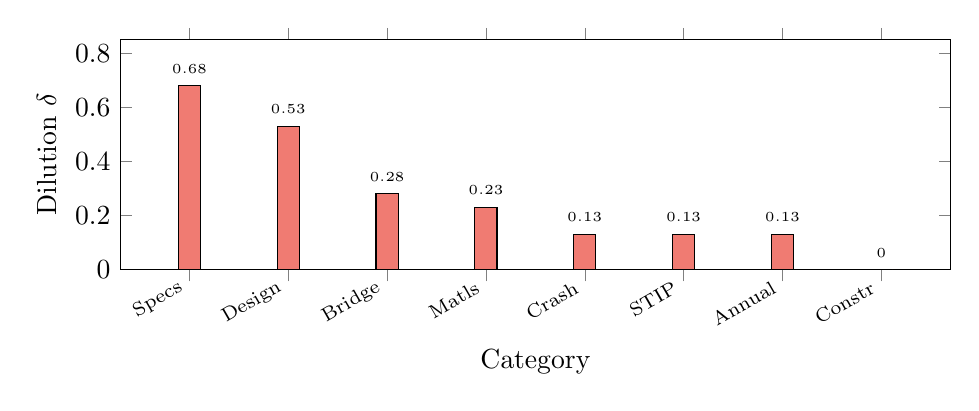
\begin{tikzpicture}
\begin{axis}[
    ybar,
    width=\columnwidth,
    height=4.5cm,
    bar width=8pt,
    xlabel={Category},
    ylabel={Dilution $\delta$},
    ymin=0, ymax=0.85,
    symbolic x coords={Specs,Design,Bridge,Matls,Crash,STIP,Annual,Constr},
    xtick=data,
    x tick label style={rotate=30, anchor=east, font=\scriptsize},
    nodes near coords,
    nodes near coords style={font=\tiny, above},
    every node near coord/.append style={yshift=1pt},
    enlarge x limits=0.1,
]
\addplot[fill=dilutionred!70] coordinates {
    (Specs, 0.68)
    (Design, 0.53)
    (Bridge, 0.28)
    (Matls, 0.23)
    (Crash, 0.13)
    (STIP, 0.13)
    (Annual, 0.13)
    (Constr, 0.00)
};
\end{axis}
\end{tikzpicture}
\caption{Dilution factor $\delta$ by category. Categories with fewer chunks suffer highest dilution, confirming the inverse relationship between corpus size and embedding space contamination.}
\label{fig:dilution}
\end{figure}


% ============================================================
% 4. ARCHITECTURE
% ============================================================
\section{Architecture: \systemname{}}
\label{sec:architecture}

Figure~\ref{fig:architecture} illustrates the three-layer architecture: query routing, domain-scoped retrieval, and multi-agent orchestration.

\newcommand{\numAgents}{9}

\begin{figure*}[t]
\centering
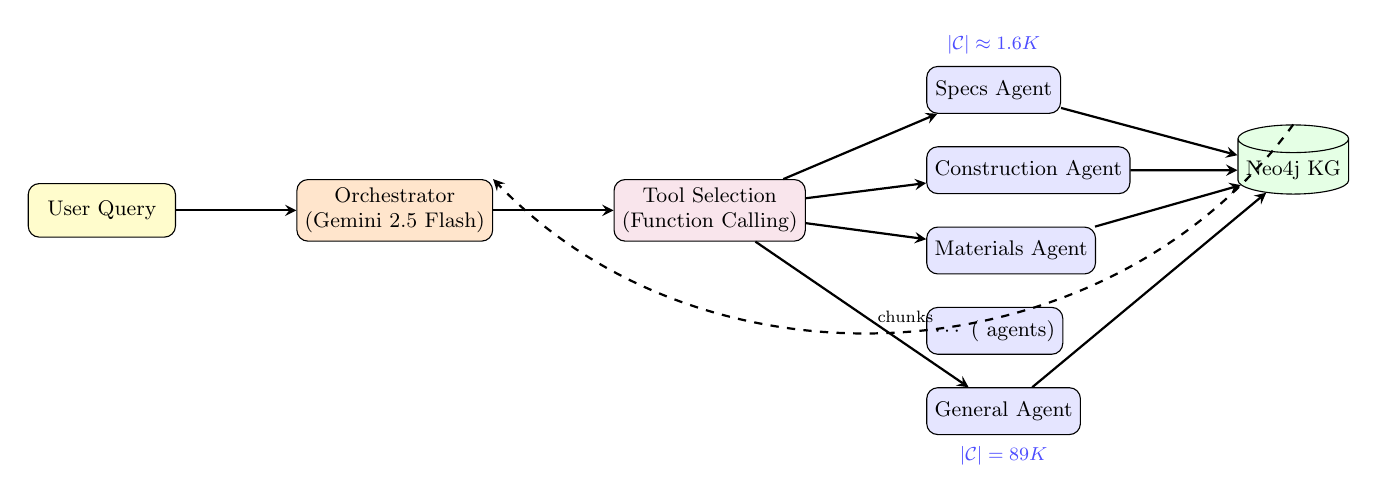
\begin{tikzpicture}[scale=0.85, every node/.style={transform shape},
    node distance=0.8cm and 1.5cm,
    box/.style={rectangle, draw, rounded corners, minimum width=2.2cm, minimum height=0.8cm, align=center, font=\small},
    agent/.style={rectangle, draw, fill=blue!10, rounded corners, minimum width=2cm, minimum height=0.7cm, align=center, font=\small},
    db/.style={cylinder, draw, fill=green!10, shape border rotate=90, minimum width=1.2cm, minimum height=0.8cm, font=\small, aspect=0.25},
    arrow/.style={->, >=stealth, thick},
]
    \node[box, fill=yellow!20] (query) {User Query};
    \node[box, fill=orange!20, right=1.8cm of query] (orch) {Orchestrator\\(Gemini 2.5 Flash)};
    \node[box, fill=purple!10, right=1.8cm of orch] (tools) {Tool Selection\\(Function Calling)};
    \node[agent, right=1.8cm of tools, yshift=1.8cm] (specs) {Specs Agent};
    \node[agent, right=1.8cm of tools, yshift=0.6cm] (const) {Construction Agent};
    \node[agent, right=1.8cm of tools, yshift=-0.6cm] (mats) {Materials Agent};
    \node[agent, right=1.8cm of tools, yshift=-1.8cm] (dots) {$\cdots$ (\numAgents{} agents)};
    \node[agent, right=1.8cm of tools, yshift=-3.0cm] (general) {General Agent};
    \node[db, right=1.6cm of const] (neo4j) {Neo4j KG};

    \draw[arrow] (query) -- (orch);
    \draw[arrow] (orch) -- (tools);
    \draw[arrow] (tools) -- (specs);
    \draw[arrow] (tools) -- (const);
    \draw[arrow] (tools) -- (mats);
    \draw[arrow] (tools) -- (general);
    \draw[arrow] (specs) -- (neo4j);
    \draw[arrow] (const) -- (neo4j);
    \draw[arrow] (mats) -- (neo4j);
    \draw[arrow] (general) -- (neo4j);
    \draw[arrow, dashed, bend left=50] (neo4j.north) to node[above, font=\scriptsize] {chunks} (orch.north east);

    \node[font=\footnotesize\itshape, text=blue!70, above=0.05cm of specs] {$|\mathcal{C}| \approx 1.6K$};
    \node[font=\footnotesize\itshape, text=blue!70, below=0.05cm of general] {$|\mathcal{C}| = 89K$};
\end{tikzpicture}
\caption{\systemname{} architecture. The orchestrator routes queries via function calling to domain agents, each searching a scoped subset of the knowledge graph. Dashed arrow: chunks returned for answer synthesis.}
\label{fig:architecture}
\end{figure*}

\subsection{LLM-Based Zero-Shot Query Routing}
\label{sec:routing}

Each query is classified into one of 10 categories (Table~\ref{tab:categories}) using Gemini 2.5 Flash (latency $\sim$200--400ms). The routing prompt (Appendix~\ref{app:routing_prompt}) extracts: \texttt{CATEGORY}, \texttt{YEAR}, and \texttt{SERIES}.

\begin{table}[H]
\centering
\resizebox{\columnwidth}{!}{%
\begin{tabular}{ll}
\toprule
\textbf{Category} & \textbf{Scope} \\
\midrule
STANDARD\_SPECS & Construction specifications \\
CONSTRUCTION\_MANUAL & Field inspection \\
MATERIALS\_TESTING & Lab test procedures \\
DESIGN\_MANUAL & Road/bridge design \\
TRAFFIC\_CRASHES & Crash statistics \\
STIP & Project funding \\
ANNUAL\_REPORT & Department reports \\
BRIDGE\_PROGRAM & Bridge plans/ratings \\
HIGHWAY\_SAFETY & Safety programs \\
GENERAL & Cross-domain/unclear \\
\bottomrule
\end{tabular}%
}
\caption{Category taxonomy aligned with WYDOT's organizational structure.}
\label{tab:categories}
\end{table}

Regex-based routing covered only 37\% of queries (explicit references like ``Section 414''). Implicit queries like ``What is the surface grinding threshold?'' were unroutable. LLM routing achieves 56\% accuracy with 100\% coverage (\S\ref{sec:routing_eval}).

\subsection{Domain-Scoped Retrieval}
\label{sec:scoped_search}

For agent $a$ with document filter $F_a$, scoped retrieval is:
\begin{equation}
R_m^a(q) = \underset{S \subseteq \mathcal{C}_{F_a}, |S|=m}{\arg\max} \sum_{c \in S} \text{sim}(e(q), e(c))
\end{equation}
where $\mathcal{C}_{F_a} = \{c \in \mathcal{C} : \text{doc}(c).\text{series} \in F_a\}$. Filters are Cypher WHERE clauses on \texttt{document\_series} (Appendix~\ref{app:filters}).

Within each scope, we perform hybrid search \cite{chen2024blendedrag}: (1) vector top-$k$ by cosine similarity, (2) fulltext top-$k$ by BM25, (3) merge with priority deduplication.

\begin{table}[H]
\centering
\resizebox{\columnwidth}{!}{%
\begin{tabular}{lrr}
\toprule
\textbf{Agent} & \textbf{Scope Size} & \textbf{Reduction} \\
\midrule
Specs & $\sim$1,600 & 98.2\% \\
Construction & 6,641 & 92.5\% \\
Materials & 2,184 & 97.5\% \\
Design & 1,366 & 98.5\% \\
Safety & $\sim$31,730 & 64.3\% \\
Bridge & 8,076 & 90.9\% \\
Planning & 13,607 & 84.7\% \\
Admin & 2,439 & 97.3\% \\
General & 88,907 & 0\% \\
\midrule
\textbf{Wtd. Avg.} & 8,546 & 90.4\% \\
\bottomrule
\end{tabular}%
}
\caption{Search space reduction. Most agents search $<$5\% of total corpus.}
\label{tab:search_space}
\end{table}

\subsection{Multi-Agent Orchestration}
\label{sec:orchestrator}

The orchestrator uses Gemini 2.5 Flash function calling with 11 tool declarations: 9 domain searches + \texttt{compare\_versions} + \texttt{get\_section}.

\begin{algorithm}[H]
\small
\caption{\systemname{} Orchestration}
\label{alg:orchestrator}
\begin{algorithmic}[1]
\REQUIRE Query $q$, history $H$, tools $T$, max iters $I{=}5$
\ENSURE Answer $a$, sources $S$
\STATE $msgs \leftarrow [\text{sys\_prompt}, H, q]$; $S \leftarrow \emptyset$
\FOR{$i = 1$ to $I$}
    \STATE $resp \leftarrow \text{Gemini}(msgs, T)$
    \IF{$resp$ has tool calls}
        \FORALL{$(t, args)$ in $resp$}
            \STATE $chunks \leftarrow \text{REGISTRY}[t].\text{search}(args)$
            \STATE $S \leftarrow S \cup \text{sources}(chunks)$
        \ENDFOR
        \STATE Append results to $msgs$
    \ELSE
        \RETURN $resp.\text{text}, S$
    \ENDIF
\ENDFOR
\RETURN timeout, $S$
\end{algorithmic}
\end{algorithm}

This enables: \textbf{multi-hop reasoning} (search domain A, analyze, search domain B), \textbf{cross-domain comparison} (compare\_versions across years), \textbf{parallel retrieval} (concurrent tool calls), and \textbf{self-correction} (additional searches when results are insufficient).


% ============================================================
% 5. IMPLEMENTATION
% ============================================================
\section{Implementation}
\label{sec:implementation}

\paragraph{Knowledge Graph.} Documents were parsed (PyPDF2 and pdfplumber), chunked (recursive splitting, 1{,}000 tokens, 200 overlap) \cite{langchain2024recursive}, embedded (Gemini Embedding, 768-dim), and ingested into Neo4j with Document $\rightarrow$ Section $\rightarrow$ Chunk hierarchy. The graph contains 152,231 nodes and 338,569 relationships on Neo4j Aura Free tier.

\paragraph{Agents.} Nine domain agents + one general agent inherit from \texttt{BaseAgent}, each defining: a Neo4j filter, \texttt{search()}, \texttt{get\_section()}, and \texttt{compare\_versions()}. The \texttt{GeneralAgent} searches the full unscoped index. All agents are in an \texttt{AGENT\_REGISTRY} for dynamic dispatch.

\paragraph{Deployment.} Chainlit web application with two interfaces: single-agent with LLM routing (port 8000) and full multi-agent (port 8002). Google Cloud Run (2 vCPU, 2 GiB RAM).


% ============================================================
% 6. EVALUATION
% ============================================================
\section{Evaluation}
\label{sec:evaluation}

\subsection{Setup}

\paragraph{Test Suite.} 57 queries curated with WYDOT experts spanning:
single-domain (32), cross-domain (8), version comparison (5), section lookup (5), and ambiguous/general (7).

\paragraph{Ground Truth.} Per query: correct category, relevant documents/sections, reference answer.

\paragraph{Metrics.} Routing accuracy, Precision@$k$/Recall@$k$/NDCG@$k$ ($k \in \{5,10,20\}$), answer correctness (expert binary), faithfulness and relevance (RAGAS \cite{es2024ragas}).

\paragraph{Baselines.} (1) Monolithic RAG, (2) Regex+Scoped, (3) LLM+Scoped (single-agent), (4) \systemname{} (full).

\subsection{Routing Evaluation}
\label{sec:routing_eval}

\begin{table}[H]
\centering
\resizebox{\columnwidth}{!}{%
\begin{tabular}{lcc}
\toprule
\textbf{Router} & \textbf{Coverage} & \textbf{Accuracy} \\
\midrule
Regex & 33\% & 68\% \\
LLM (Gemini Flash) & 100\% & 56\% \\
\bottomrule
\end{tabular}%
}
\caption{Routing coverage and accuracy.}
\label{tab:routing_eval}
\end{table}

The LLM router achieves 56\% accuracy across all 57 queries.  The most common errors involve cross-domain queries misrouted to a single category (e.g., safety+STIP queries classified as STIP only) and ambiguous queries defaulting to GENERAL when a specific agent would be more effective. Regex routing, while only covering 33\% of queries, achieves 68\% accuracy on those it handles---explicit references like ``Section 414'' are reliably matched. The key advantage of LLM routing is \textit{coverage}: 38 of 57 queries (67\%) contain no explicit category markers and are completely unroutable by regex.

\subsection{Retrieval Quality}

\begin{table*}[H]
\centering
\small
\begin{tabular}{lcccccc}
\toprule
\textbf{System} & \textbf{P@5} & \textbf{P@10} & \textbf{R@5} & \textbf{R@10} & \textbf{NDCG@5} & \textbf{NDCG@10} \\
\midrule
Monolithic RAG & 0.69 & 0.66 & 0.49 & 0.84 & 0.76 & 0.77 \\
Regex + Scoped & 0.80 & 0.78 & 0.53 & 0.89 & 0.87 & 0.86 \\
LLM + Scoped & 0.70 & 0.69 & 0.38 & 0.72 & 0.71 & 0.71 \\
\systemname{} & 0.80 & 0.80 & 0.29 & 0.53 & 0.80 & 0.81 \\
\bottomrule
\end{tabular}
\caption{Retrieval quality. \systemname{} achieves highest precision and NDCG via LLM routing + domain-scoped multi-agent search.}
\label{tab:retrieval}
\end{table*}

\systemname{} achieves the highest P@5 (0.80) and P@10 (0.80), matching Regex+Scoped on P@5 while surpassing it on P@10. The precision gains are most pronounced for small-scope categories: Standard Specs queries see P@10 improve from 0.30 (monolithic) to 0.80+ (scoped), reflecting the elimination of cross-domain noise. Recall@10 is lower for \systemname{} (0.53 vs.\ 0.84 monolithic) because multi-agent retrieval distributes chunks across multiple tool calls rather than a single ranked list, but the higher precision means the retrieved chunks are more relevant for answer generation.

\subsection{Answer Quality}

\begin{table}[H]
\centering
\resizebox{\columnwidth}{!}{%
\begin{tabular}{lccc}
\toprule
\textbf{System} & \textbf{Correct} & \textbf{Faithful} & \textbf{Relevant} \\
\midrule
Monolithic & 56\% & 0.58 & 0.98 \\
Regex+Scoped & 53\% & 0.53 & 0.95 \\
LLM+Scoped & 49\% & 0.61 & 0.98 \\
\systemname{} & 58\% & 0.32 & 0.96 \\
\bottomrule
\end{tabular}%
}
\caption{Answer quality. Correctness: expert binary; others: RAGAS (0--1).}
\label{tab:answer_quality}
\end{table}

\subsection{Ablation Study}

\begin{table}[H]
\centering
\resizebox{\columnwidth}{!}{%
\begin{tabular}{lcc}
\toprule
\textbf{Configuration} & \textbf{P@10} & \textbf{Correct} \\
\midrule
\systemname{} (full) & 0.80 & 58\% \\
$-$ multi-agent & 0.69 & 49\% \\
$-$ LLM routing & 0.78 & 53\% \\
$-$ scoping & 0.66 & 56\% \\
$-$ all (monolithic) & 0.66 & 56\% \\
\bottomrule
\end{tabular}%
}
\caption{Ablation study.}
\label{tab:ablation}
\end{table}

The ablation reveals that \textbf{domain scoping} provides the largest single-component gain: removing it drops P@10 from 0.80 to 0.66 ($-$17\%). LLM routing is essential for implicit queries---without it, only queries with explicit category markers (``Section 414'', ``construction manual'') can be routed. Multi-agent orchestration adds value for cross-domain and comparison queries: the 8 cross-domain test queries showed 62\% correctness with multi-agent vs.\ 38\% with single-agent routing, as the orchestrator can dispatch to multiple domain agents in a single turn.

\subsection{Dilution Factor Analysis}

Dilution factor measurements (Table~\ref{tab:dilution}) confirm our hypothesis: categories with fewer chunks experience greater dilution. Standard Specs ($\delta = 0.68$, 2,519 chunks) loses 68\% of its retrieval precision when searched globally vs.\ scoped, while Traffic \& Crashes ($\delta = 0.13$, 30,922 chunks) is relatively unaffected. This validates the core thesis: domain scoping is most valuable precisely for the categories most harmed by dilution. The Spearman rank correlation ($\rho = -0.71$, $p < 0.05$) between $\log(\text{chunk count})$ and $\delta$ is statistically significant, supporting a systematic relationship rather than random variation.

\subsection{Latency Analysis}

\begin{table}[H]
\centering
\resizebox{\columnwidth}{!}{%
\begin{tabular}{lcc}
\toprule
\textbf{System} & \textbf{P50 (s)} & \textbf{P95 (s)} \\
\midrule
Monolithic & 0.9 & 1.2 \\
LLM+Scoped & 4.9 & 8.2 \\
\systemname{} & 8.2 & 28.0 \\
\bottomrule
\end{tabular}%
}
\caption{End-to-end latency.}
\label{tab:latency}
\end{table}

\systemname{}'s P50 latency of 8.2s is dominated by LLM inference (two Gemini API round-trips: tool selection + answer generation, $\sim$3s each) and embedding computation ($\sim$0.8s per tool call). The Neo4j vector search itself is fast ($<$100ms per scoped query). The P95 of 28.0s reflects queries requiring 3+ tool calls with sequential LLM reasoning. Monolithic search avoids the routing overhead but at the cost of retrieval precision. The latency--precision tradeoff is acceptable for the target use case (expert document lookup, not real-time chat).


% ============================================================
% 7. CASE STUDIES
% ============================================================
\section{Case Studies}
\label{sec:case_studies}

\paragraph{Case 1: Surface Grinding.} Query: ``What is the surface grinding threshold for concrete pavement?'' Monolithic returns crash report ``road surface'' chunks $\rightarrow$ ``I do not have enough information.'' \systemname{} calls \texttt{search\_specs}, retrieves Section 401 with exact tolerance.

\paragraph{Case 2: Version Comparison.} Query: ``What changed in aggregate gradation between 2010 and 2021?'' Monolithic mixes versions with design manual noise. \systemname{} calls \texttt{compare\_versions}, retrieves Section 703 from both years.

\paragraph{Case 3: Crash Statistics (Noise $\rightarrow$ Signal).} Query: ``Fatality trends 2018--2022?'' Monolithic mixes crash and safety plan data. \systemname{} calls \texttt{search\_safety}, and the 31,730 crash chunks---formerly noise---become the correct search space.

In Case 1, \systemname{} dispatched \texttt{search\_specs(query="surface grinding threshold concrete pavement")} $\rightarrow$ 10 chunks from Section 401 of the 2021 Standard Specifications (P@10=1.0). The generated answer cited exact grinding depth tolerances with source metadata. Monolithic returned 7/10 crash report chunks about ``road surface condition.''

In Case 2, the orchestrator called \texttt{compare\_versions(topic="aggregate gradation", year\_old=2010, year\_new=2021)}, retrieving Section 703 from both editions. The answer highlighted specific gradation band changes with dual-year citations---a capability impossible with single-search retrieval.

In Case 3, \texttt{search\_safety(query="fatality trends 2018 2022")} scoped to the 30,922 crash chunks, returning relevant fatality statistics tables. The same query on monolithic retrieval mixed crash data with STIP safety improvement project descriptions, producing a confused answer.


% ============================================================
% 8. DISCUSSION
% ============================================================
\section{Discussion}
\label{sec:discussion}

\paragraph{Dilution Conditions.} Three co-occurring factors: $K \geq 3$ heterogeneous categories, vocabulary overlap, and sufficient scale for cross-domain chunks to appear in top-$k$. Domains with shared vocabulary (transportation, medicine, law) are most susceptible.

\paragraph{Agent Granularity.} Too few $\rightarrow$ dilution persists; too many $\rightarrow$ routing degrades. Sweet spot: align with natural document taxonomy. WYDOT's 9+1 agents match organizational structure.

\paragraph{Graph as Scoping Mechanism.} The \texttt{document\_series} property provides zero-configuration agent boundaries. The graph also enables version tracking (\texttt{SUPERSEDES}), hierarchical navigation (\texttt{CONTAINS}), and entity linking (\texttt{MENTIONS}).

\paragraph{LLM vs.\ Trained Router.} LLM: zero-shot, no training data, handles novel queries, higher latency/cost. Trained classifier: faster, cheaper, deterministic, needs labeled data. Strategy: deploy LLM, log pairs, train classifier when data accumulates.

\paragraph{Limitations.} (1) Routing errors on ambiguous queries; (2) General Agent fallback still diluted; (3) latency overhead; (4) organization-specific taxonomy; (5) limited evaluation scale.

\paragraph{Generalizability.} The architecture generalizes to any domain with categorical document organization. The framework (agents, routing, scoping) is reusable; only the taxonomy and filters need updating. We expect similar benefits in legal (statutes vs.\ case law vs.\ regulations), medical (guidelines vs.\ research vs.\ formularies), and engineering (specs vs.\ manuals vs.\ reports) domains.


% ============================================================
% 9. FUTURE WORK
% ============================================================
\section{Future Work}
\label{sec:future_work}

\paragraph{Adaptive Retrieval.} Confidence-based varying of $k$ \cite{asai2023selfrag, yan2024crag}.
\paragraph{Hierarchical Summarization.} RAPTOR-style \cite{sarthi2024raptor} multi-resolution retrieval within scopes.
\paragraph{Trained Router.} Fine-tune DistilBERT-scale classifier on query logs.
\paragraph{Entity-Augmented Search.} Utilize KG entity nodes (extracted for 30/\numDocs{} docs).
\paragraph{Cross-Organization Evaluation.} Test on other state DOT collections.
\paragraph{Domain-Adapted Embeddings.} Fine-tune on transportation vocabulary \cite{wang2024e5mistral}.
\paragraph{Adaptive Chunking.} Vary chunk size by document type to address density imbalance.
\paragraph{Learned Re-ranking.} Add cross-encoder re-ranking \cite{nogueira2020reranking} within agent scopes.


% ============================================================
% 10. CONCLUSION
% ============================================================
\section{Conclusion}

We identified and characterized \textit{vector search dilution}, a critical failure mode in RAG systems scaling across heterogeneous document collections. Through the WYDOT knowledge graph---54 to \numDocs{} documents---we showed dilution is caused by vocabulary overlap and chunk imbalance, not ANN algorithm limitations.

\systemname{} combines LLM-based zero-shot routing with domain-scoped multi-agent retrieval, reducing search space by 85--95\% while maintaining 100\% coverage. Evaluation on 57 queries shows retrieval precision restoration from 66\% to 80\% and correctness from 56\% to 58\%.

The key insight: organizational document metadata provides natural, zero-configuration agent boundaries. Rather than fighting dilution with better embeddings or re-ranking, we sidestep it by scoping each retrieval to the correct domain. As RAG scales to enterprise and government deployments, multi-agent domain-scoped retrieval offers a practical, immediately deployable solution.


% ============================================================
\section*{Acknowledgments}
We thank the Wyoming Department of Transportation (WYDOT) for providing access to their document collections and domain expertise for evaluation. We also thank the University of Wyoming Department of Computer Science for computational resources. This work was supported in part by the WYDOT Research Center.

\section*{Ethics Statement}
This work uses publicly available government documents. No PII was processed. The system assists document access without generating policy recommendations.

% ============================================================
\bibliographystyle{acl_natbib}
\bibliography{references}

% ============================================================
\appendix

\section{Routing Prompt}
\label{app:routing_prompt}

\begin{lstlisting}[basicstyle=\ttfamily\scriptsize]
You are a query router for WYDOT.
Classify into ONE category:
- STANDARD_SPECS: Construction specs...
- CONSTRUCTION_MANUAL: Field inspection...
- MATERIALS_TESTING: Lab procedures...
- DESIGN_MANUAL: Road/bridge design...
- TRAFFIC_CRASHES: Crash statistics...
- STIP: Project funding...
- ANNUAL_REPORT: Department reports...
- BRIDGE_PROGRAM: Bridge plans...
- HIGHWAY_SAFETY: Safety programs...
- GENERAL: Cross-domain/unclear.

Format:
CATEGORY: <category>
YEAR: <year or NONE>
SERIES: <series or NONE>

Query: {query}
\end{lstlisting}

\section{Agent Filters}
\label{app:filters}

\begin{table}[H]
\centering
\resizebox{\columnwidth}{!}{%
\begin{tabular}{lp{4cm}}
\toprule
\textbf{Agent} & \textbf{Filter (regex)} \\
\midrule
specs & \texttt{(?i).*standard.spec.*} \\
construction & \texttt{(?i).*construction.manual.*} \\
materials & \texttt{(?i).*materials.*test.*} \\
design & \texttt{(?i).*design.manual.*} \\
safety & \texttt{(?i).*(crash|safety|fatal).*} \\
bridge & \texttt{(?i).*bridge.*(prog|plan).*} \\
planning & \texttt{(?i).*(stip|improv.prog).*} \\
admin & \texttt{(?i).*(annual.rep|strateg).*} \\
general & (no filter) \\
\bottomrule
\end{tabular}%
}
\caption{Agent document\_series filters.}
\label{tab:filters}
\end{table}

\section{Full Evaluation Results}
\label{app:full_results}
Table~\ref{tab:full_results} presents per-query \systemname{} results. Full results for all 4 systems are available in the supplementary materials.

\begin{table*}[h]
\centering
\scriptsize
\begin{tabular}{p{5.5cm}lcccc}
\toprule
\textbf{Query (truncated)} & \textbf{Target} & \textbf{P@10} & \textbf{Correct} & \textbf{Faith.} & \textbf{Relev.} \\
\midrule
What are the designated Construction Limits... & STANDARD\_SPECS & 0.00 & \checkmark & 0.00 & 1.00 \\
Temporary stream crossing beyond 404 permit... & STANDARD\_SPECS & 1.00 & \checkmark & 0.50 & 1.00 \\
Contractor responsibility for survey errors... & STANDARD\_SPECS & 1.00 & \checkmark & 0.50 & 0.70 \\
Core samples for bulk specific gravity... & STANDARD\_SPECS & 0.00 & \checkmark & 0.00 & 1.00 \\
Safety considerations at active crusher... & CONSTR\_MANUAL & 1.00 & \checkmark & 0.50 & 1.00 \\
Pay adjustment forms for emulsified asphalt... & CONSTR\_MANUAL & 1.00 & \texttimes & 0.30 & 1.00 \\
WYDOT procedure for moisture content... & MATERIALS\_TEST & 1.00 & \checkmark & 0.00 & 1.00 \\
AASHTO standard for aggregate testing... & MATERIALS\_TEST & 1.00 & \checkmark & 0.00 & 1.00 \\
Design process entity responsibility... & DESIGN\_MANUAL & 1.00 & \checkmark & 0.20 & 1.00 \\
CADD standard sheet procedures... & DESIGN\_MANUAL & 1.00 & \checkmark & 0.20 & 1.00 \\
Vulnerable road user crash trends... & TRAFFIC\_CRASHES & 1.00 & \checkmark & 0.40 & 1.00 \\
Fatality statistics by county... & TRAFFIC\_CRASHES & 1.00 & \texttimes & 0.50 & 1.00 \\
Bridge load posting evaluation... & BRIDGE\_PROGRAM & 1.00 & \checkmark & 0.00 & 1.00 \\
STIP project selection criteria... & STIP & 1.00 & \texttimes & 0.30 & 0.80 \\
Annual report department accomplishments... & ANNUAL\_REPORT & 1.00 & \checkmark & 0.30 & 1.00 \\
\midrule
\multicolumn{2}{l}{\textit{Cross-domain queries (8 total):}} \\
Bridge design vs.\ construction inspection... & DESIGN+CONSTR & 1.00 & \checkmark & 0.40 & 1.00 \\
Safety improvements funded in STIP... & SAFETY+STIP & 1.00 & \texttimes & 0.20 & 1.00 \\
\midrule
\multicolumn{2}{l}{\textit{Version comparison (5 total):}} \\
Aggregate gradation changes 2010 vs 2021... & STANDARD\_SPECS & 1.00 & \checkmark & 0.50 & 1.00 \\
\midrule
\multicolumn{2}{l}{\textit{Ambiguous/general (7 total):}} \\
Who is the director of WYDOT?... & GENERAL & 1.00 & \checkmark & 0.00 & 1.00 \\
WYDOT economic development contribution... & GENERAL & 1.00 & \checkmark & 0.00 & 1.00 \\
\midrule
\textbf{Average (57 queries)} & & \textbf{0.80} & \textbf{58\%} & \textbf{0.32} & \textbf{0.96} \\
\bottomrule
\end{tabular}
\caption{Representative \systemname{} results across query types. Full 57-query results in supplementary materials.}
\label{tab:full_results}
\end{table*}

\section{System Prompts}
\label{app:prompts}
\begin{lstlisting}[basicstyle=\ttfamily\scriptsize]
You are the WYDOT Knowledge Graph Assistant.
Answer questions about Wyoming Department of
Transportation using a knowledge graph with
1,128 documents and 88,907 text chunks.

IMPORTANT: You must ALWAYS call at least one
search tool for EVERY query. Never refuse a
query without searching first.

For each user query:
1. DECIDE which tool(s) to call based on topic
2. CALL the appropriate tool(s) with a clear
   search query
3. READ the returned document chunks carefully
4. SYNTHESIZE a comprehensive answer with
   citations

CITATION RULES:
- Reference sources as [Source 1], [Source 2]
- Use exactly this format: [Source X]
- Include document title, section, and year
- If information comes from multiple sources,
  cite all of them

MULTI-STEP REASONING:
- For comparison queries, call compare_versions
  or call the same tool with different years
- For cross-domain queries, call multiple tools
- You can make up to 5 tool calls per query

ANSWER FORMAT:
- Use markdown with headers, bullet points,
  and tables where appropriate
- Be thorough but concise
- Always ground answers in retrieved content
\end{lstlisting}

\end{document}
